\normalsize
\subsection{Staggered Spatial Discretization}
The model with staggered spatial discretization is developed on a Cartesian grid system with staggered arrangement of velocities. The scalar variables are defined in the center of the cell and the velocities at the middle of cell faces. The subscript
$i, \ j, and \ k$ mean that the value is located at $(x,y,z)=(  i
\Delta x, j \Delta y, k \Delta z )$ and are different from the Einstein notation.
\begin{figure}[h]
\hspace{0.1in}
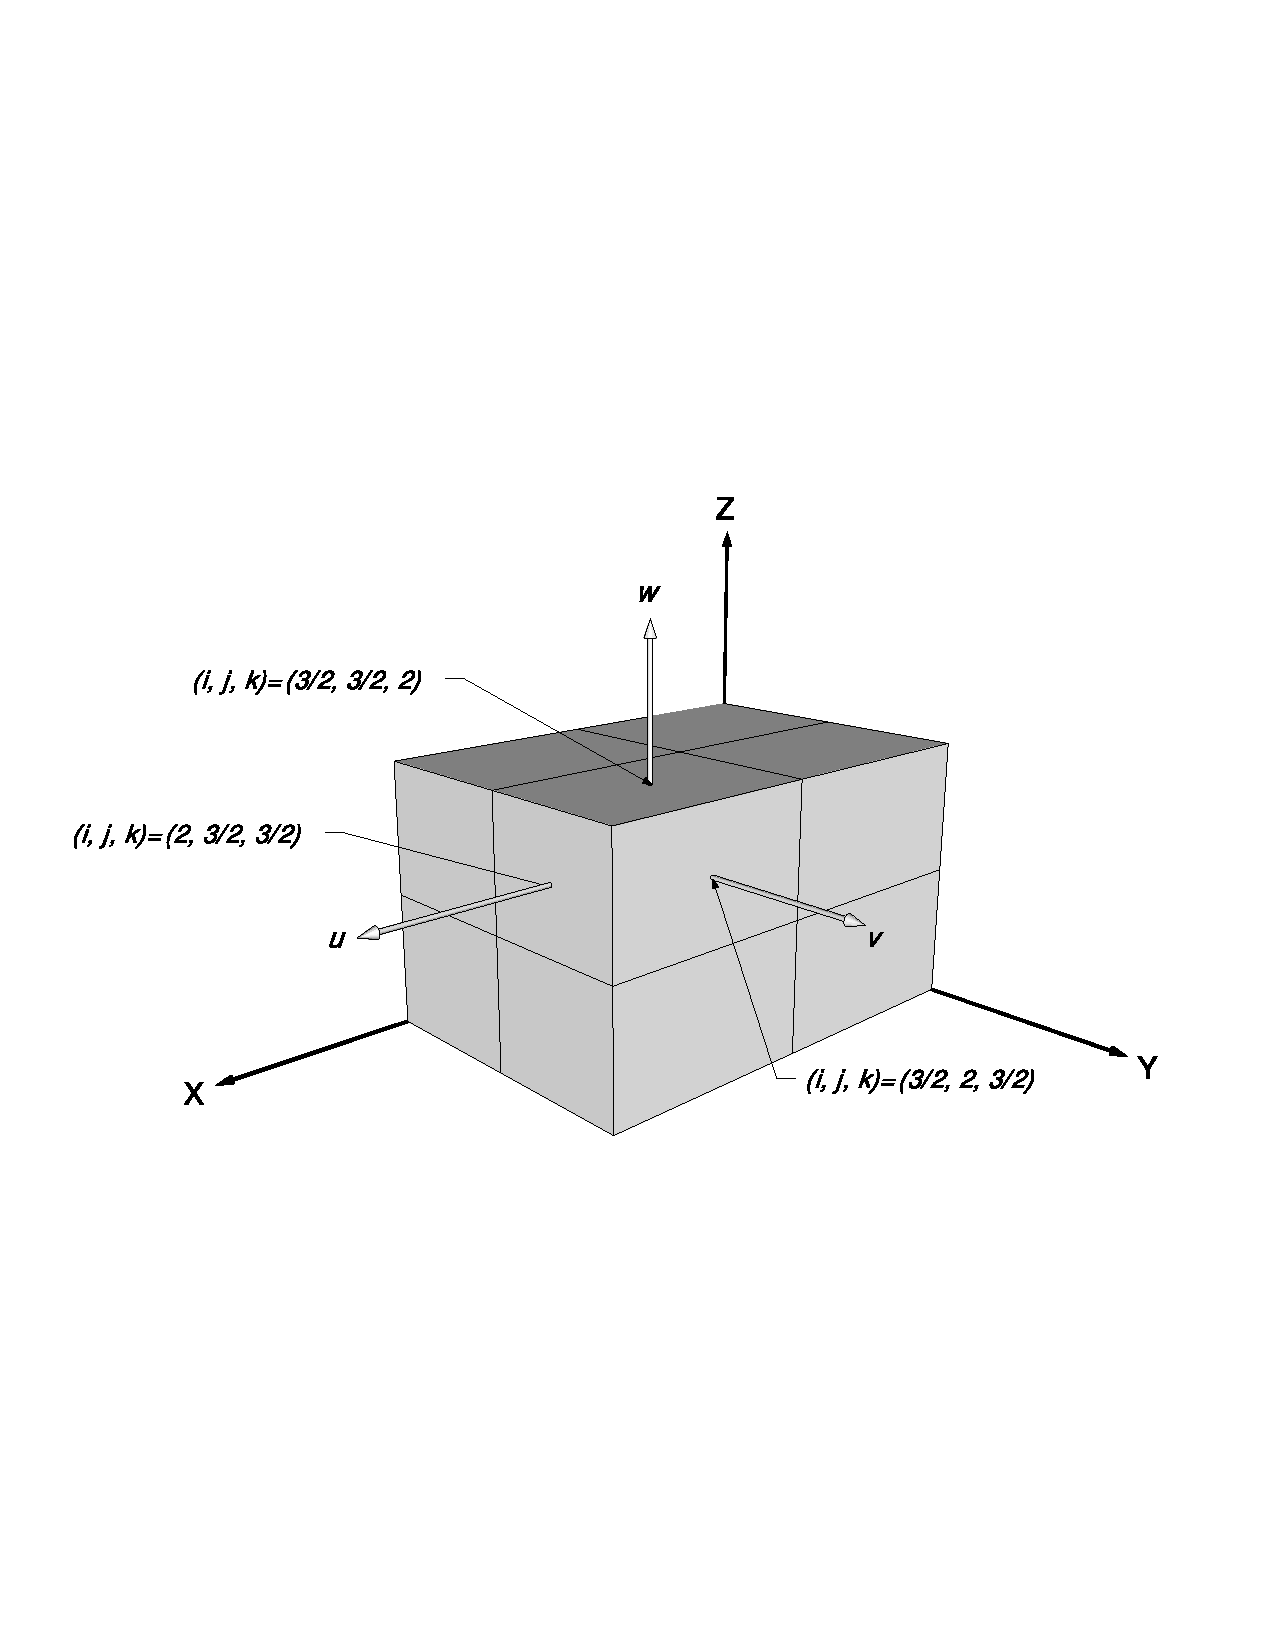
\includegraphics[width=5.6in]{../figures/Staggered/Staggered3D.pdf}
\label{fig:Staggered3D}
\caption{Staggered grid.}
\end{figure}
\begin{figure}[htbp]
\hspace{-0.1in}
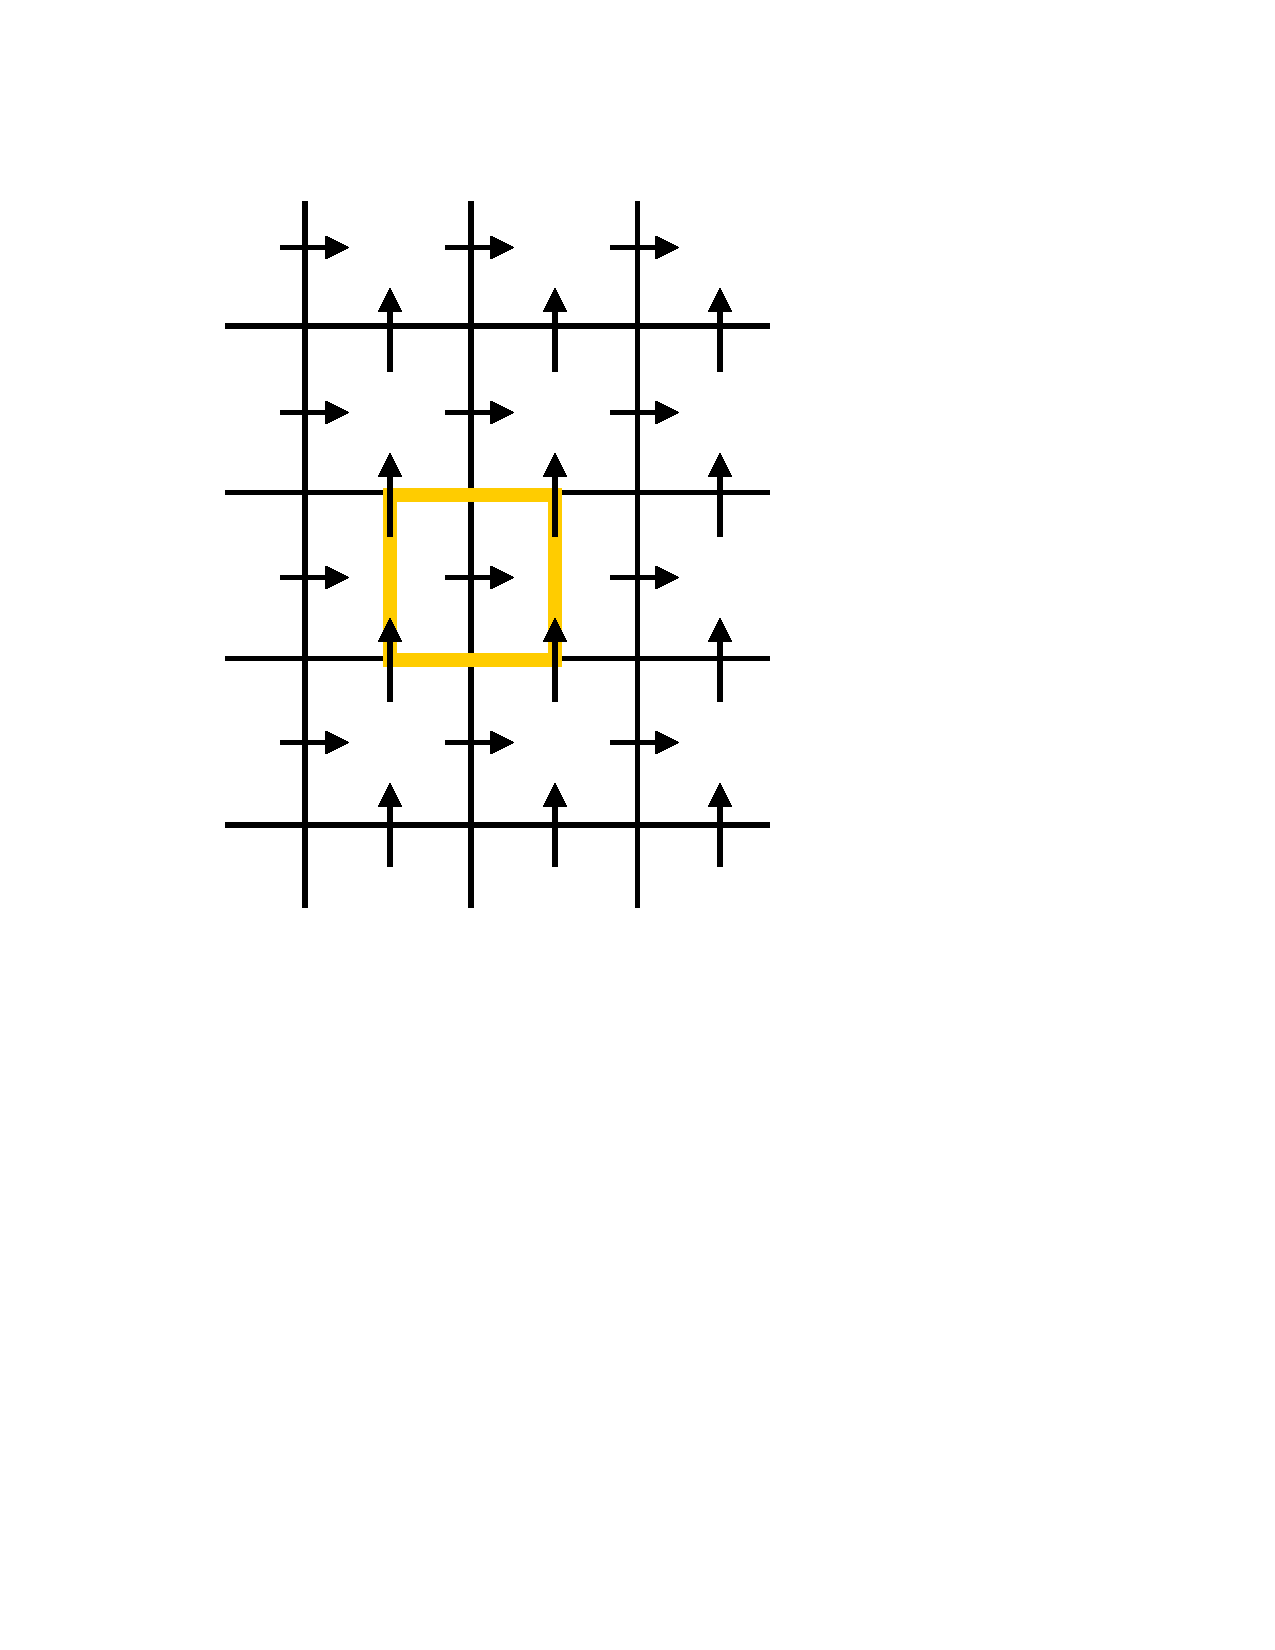
\includegraphics[scale=0.47]{../figures/Grids/Staggered-CV-u.pdf}
\hspace{0.3in}
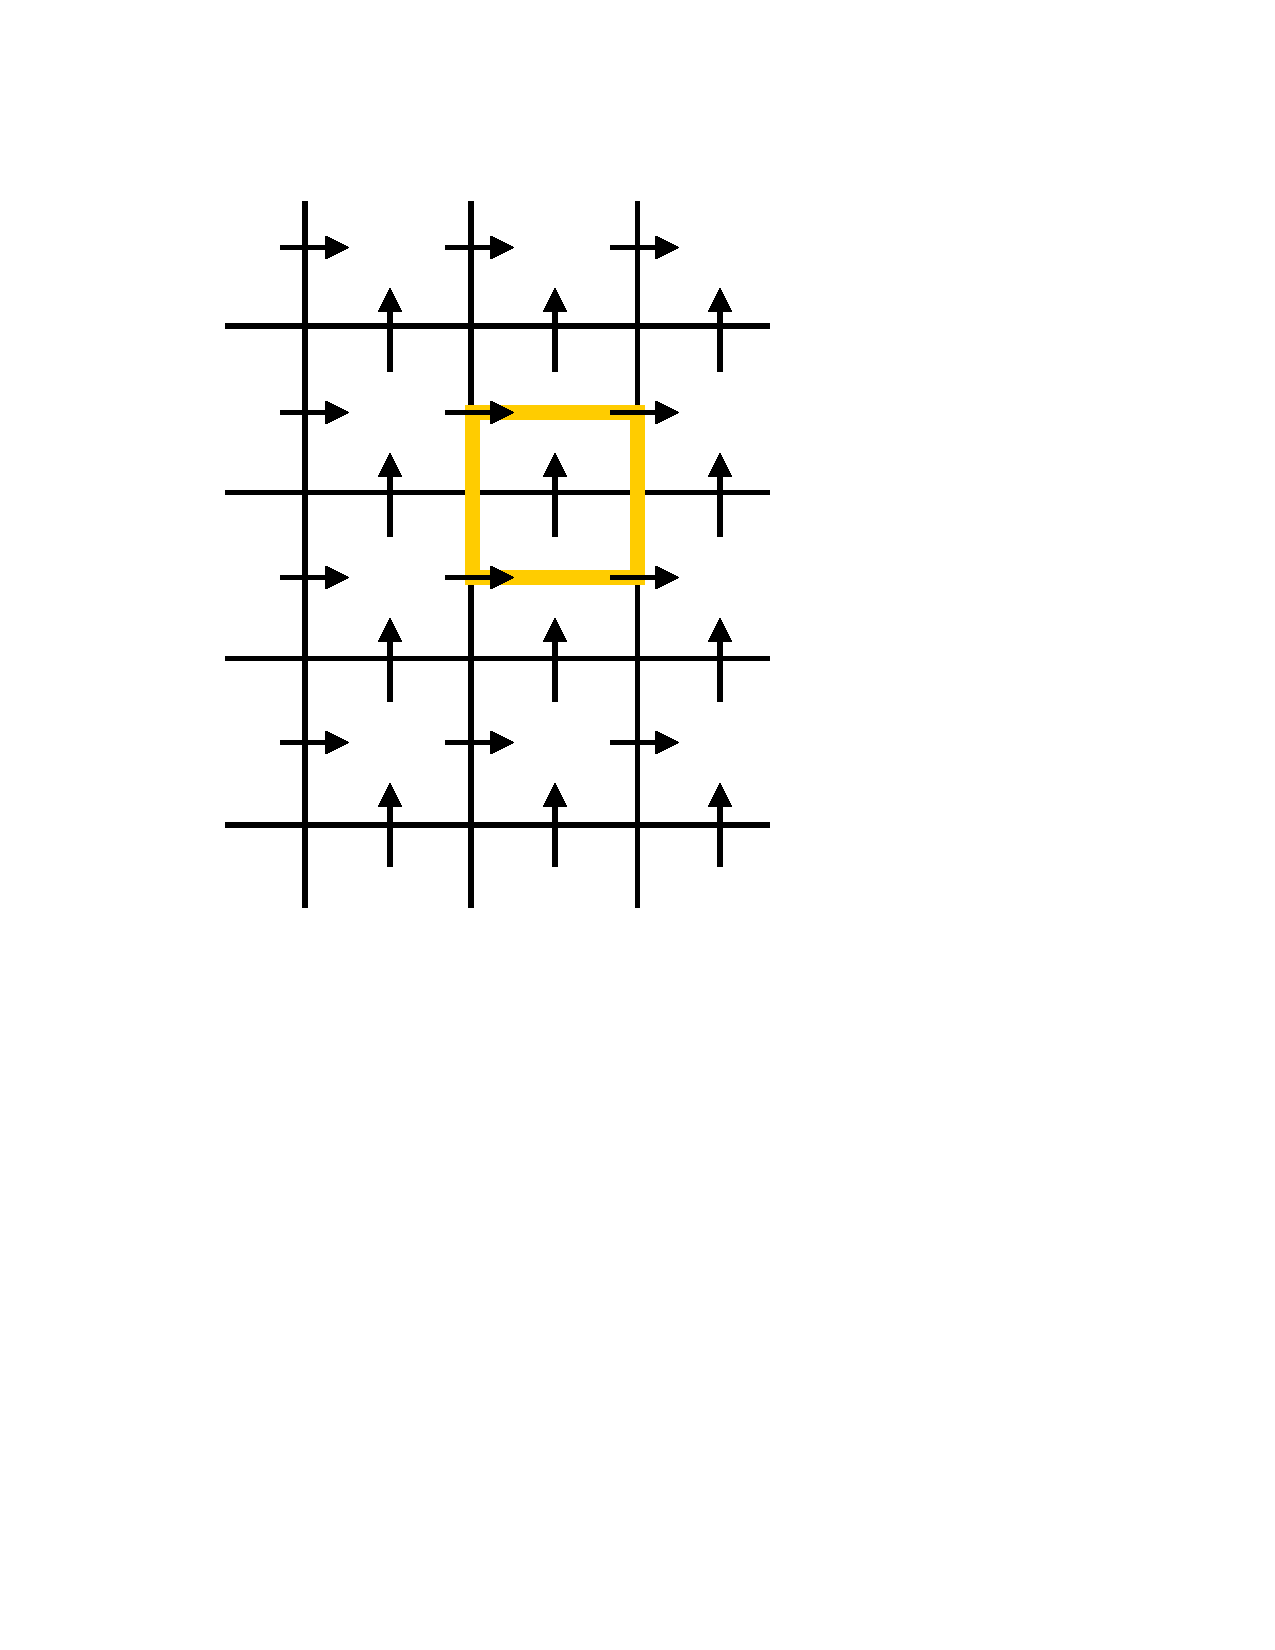
\includegraphics[scale=0.47]{../figures/Grids/Staggered-CV-w.pdf}
\hspace{0.3in}
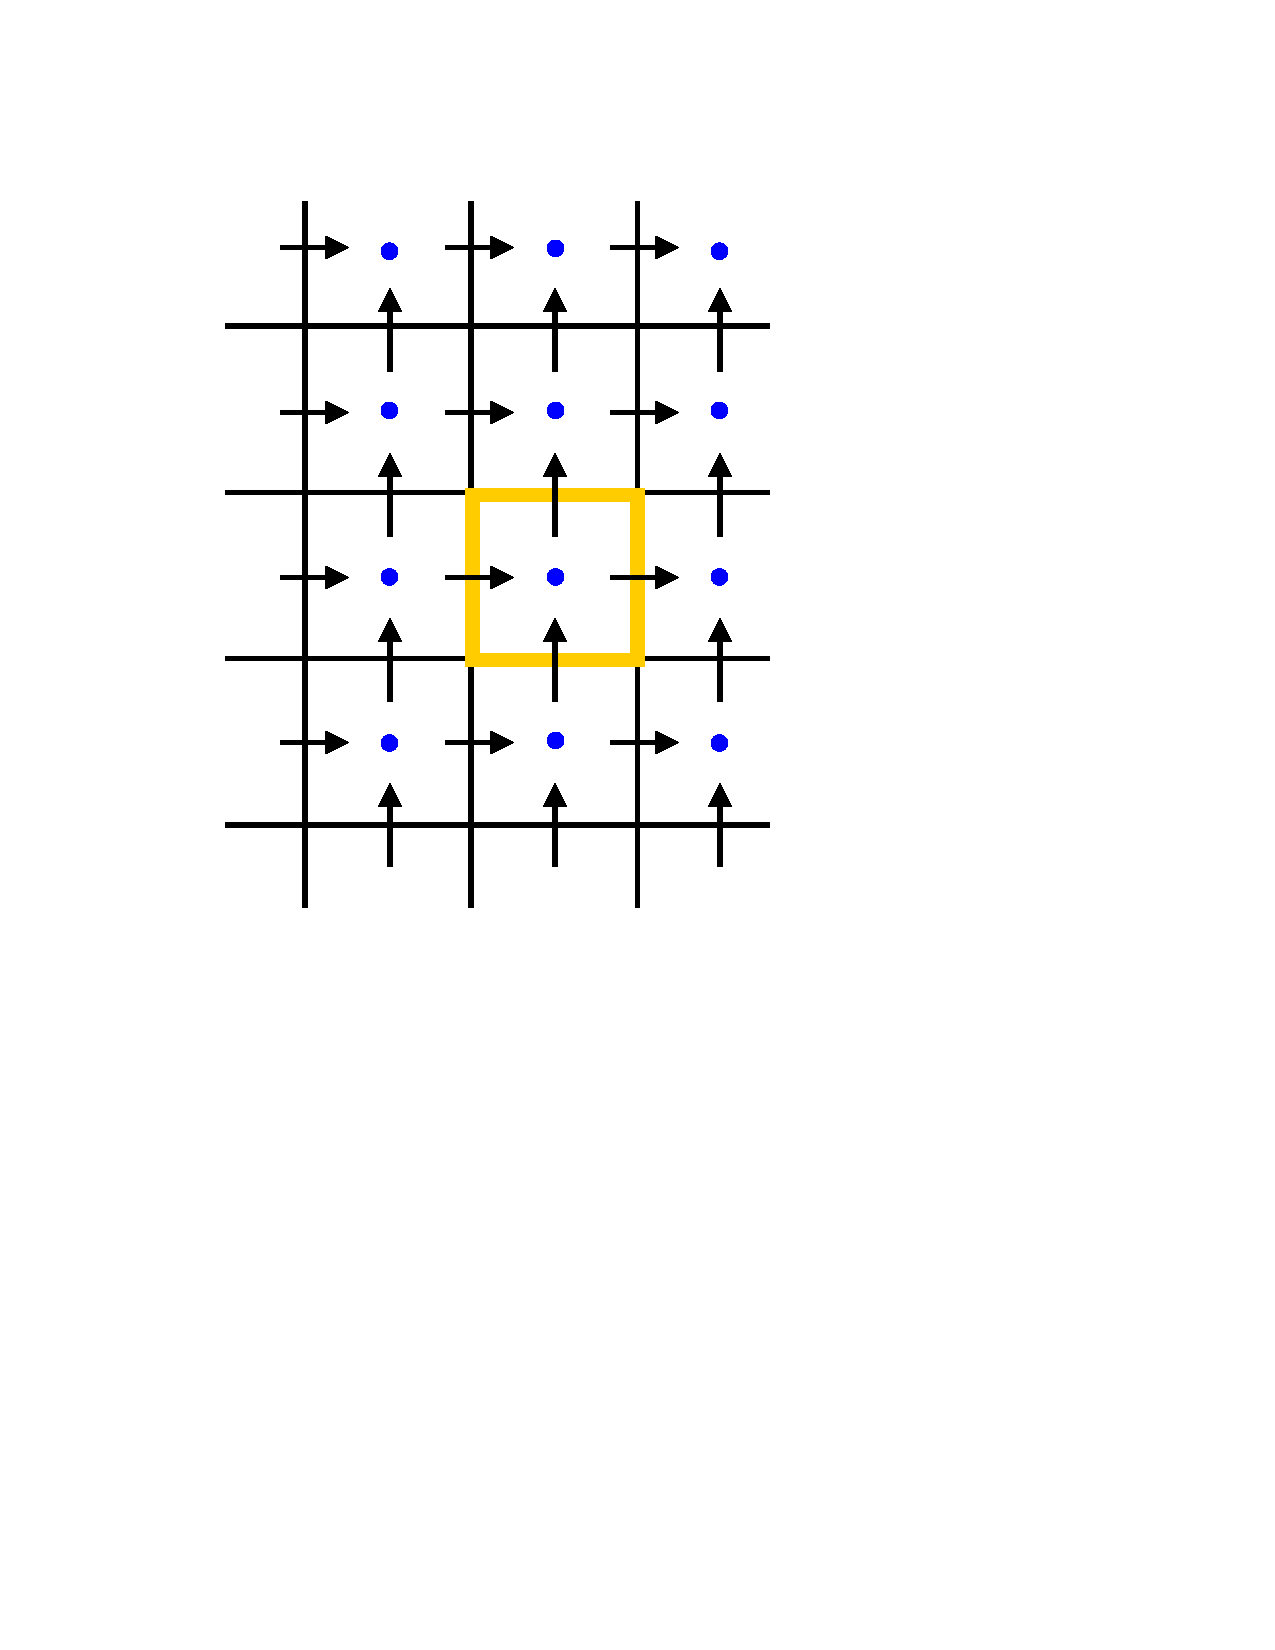
\includegraphics[scale=0.47]{../figures/Grids/Staggered-CV-scalar.pdf}
\label{fig:Staggered-CV-u}
\caption{Control volumes of the staggered grid. horizontal velocity, vertical velocity, and cell-centered scalar.}
\end{figure}
With the location of the velocities denoted by the subscript, Equation \ref{eqn:chap-FlowModel-momentum-u}, \ref{eqn:chap-FlowModel-momentum-v}, and \ref{eqn:chap-FlowModel-momentum-w} can be discretized as:
\begin {eqnarray}
u_{i+ \frac{1}{2},j,k}^{*} = u_{i+ \frac{1}{2},j,k}^{n}+ \Delta t
\{ -A(u_{i+ \frac{1}{2},j,k}^n)+E(u_{i+ \frac{1}{2},j,k}^n) \nonumber \\
-B(u_{i+
\frac{1}{2},j,k}^n)-g\frac{h_{i+1,j,k}^n-h_{i,j,k}^n}{\Delta x}
-\frac{1}{\rho}\frac{p_{d \ i+1,j,k}^n-p_{d \ i,j,k}^n}{ \Delta x}
\}
\end{eqnarray}
\begin {eqnarray}
v_{i,j+ \frac{1}{2},k}^{*} = v_{i,j+ \frac{1}{2},k}^{n}+ \Delta t
\{ -A(v_{i,j+ \frac{1}{2},k}^n)+E(v_{i,j+ \frac{1}{2},k}^n) \nonumber \\
-B(v_{i,j+
\frac{1}{2},k}^n)-g\frac{h_{i,j+1,k}^n-h_{i,j,k}^n}{\Delta y}
-\frac{1}{\rho}\frac{p_{d \ i,j+1,k}^n-p_{d \ i,j,k}^n}{ \Delta y}
\}
\end{eqnarray}
\begin {eqnarray}
w_{i,j,k+ \frac{1}{2}}^{*} = w_{i,j,k+ \frac{1}{2}}^{n}+ \Delta t
\{ -A(w_{i,j,k+ \frac{1}{2}}^n)+E(w_{i,j,k+ \frac{1}{2}}^n) \nonumber \\
-\frac{1}{\rho}\frac{p_{d \ i,j,k+1}^n-p_{d \ i,j,k}^n}{ \Delta z}
\}
\end{eqnarray}
The advection term is approximated by the central difference,
\begin{eqnarray}
A(u_{i+ \frac{1}{2} ,j,k})&=&( \frac{\partial uu}{\partial x} +  \frac{\partial
uv}{\partial y}+\frac{\partial uw}{\partial z})_{i+ \frac{1}{2} ,j, k}\nonumber\\
&=&\frac{(u^n_{i+1,j,k})^2-(u^n_{i,j,k})^2}{\Delta
x}+\frac{(uv)^n_{i+ \frac{1}{2} ,j+ \frac{1}{2} ,k}-(uv)^n_{i+
\frac{1}{2} ,j- \frac{1}{2} ,k}}{\Delta
y}\nonumber \\
& & + \frac{(uw)^n_{i+ \frac{1}{2} ,j,k + \frac{1}{2}} -(uw)^n_{i+
\frac{1}{2} ,j,k-1/2}}{\Delta z}
\end{eqnarray}
where the cell-centered velocity is approximated by the average of
neighboring points:
\begin{eqnarray*}
u^n_{i+1,j,k}&=&\frac{1}{2}(u^n_{i + \frac{3}{2},j,k}+u^n_{i+ \frac{1}{2} ,j,k})\\
u^n_{i,j,k}&=&\frac{1}{2}(u^n_{i+ \frac{1}{2} ,j,k}+u^n_{i-
\frac{1}{2} ,j,k})
\end{eqnarray*}
\begin{eqnarray*}
(uv)^n_{i+ \frac{1}{2} ,j+ \frac{1}{2} ,k}&=&\frac{1}{2}(u^n_{i+
\frac{1}{2} ,j,k}+u^n_{i+ \frac{1}{2} ,j+1,k})
\cdot \frac{1}{2}(v^n_{i,j+ \frac{1}{2} ,k}+v^n_{i+1,j+ \frac{1}{2} ,k})\\
(uv)^n_{i+ \frac{1}{2} ,j- \frac{1}{2} ,k}&=&\frac{1}{2}(u^n_{i+
\frac{1}{2} ,j,k}+u^n_{i+ \frac{1}{2} ,j-1,k}) \cdot
\frac{1}{2}(v^n_{i,j- \frac{1}{2} ,k}+v^n_{i+1,j- \frac{1}{2} ,k})
\end{eqnarray*}
\begin{eqnarray*}
(uw)^n_{i+ \frac{1}{2} ,j ,k+ \frac{1}{2}}&=&\frac{1}{2}(u^n_{i+
\frac{1}{2} ,j,k}+u^n_{i+ \frac{1}{2} ,j,k+1}) \cdot
\frac{1}{2}(w^n_{i,j ,k+ \frac{1}{2}}+w^n_{i+1,j ,k+
\frac{1}{2}})\\ (uw)^n_{i+ \frac{1}{2} ,j ,k-
\frac{1}{2}}&=&\frac{1}{2}(u^n_{i+ \frac{1}{2} ,j,k}+u^n_{i+
\frac{1}{2} ,j,k-1}) \cdot \frac{1}{2}(w^n_{i,j ,k-
\frac{1}{2}}+w^n_{i+1,j ,k- \frac{1}{2}})
\end{eqnarray*}
 The diffusion, barotropic, and baroclinic terms are:
\begin{eqnarray}
E(u_{i+ \frac{1}{2} ,j,k}) &=& \frac{\mu_h}{\Delta x^2} (u_{i +
\frac{3}{2},
j,k}-2u_{i+ \frac{1}{2} ,j,k} + u_{i- \frac{1}{2} , j,k})\nonumber \\
&+& \frac{\mu_h}{\Delta y^2} (u_{i + \frac{1}{2},
j+1,k}-2u_{i+ \frac{1}{2} ,j,k} + u_{i+ \frac{1}{2} ,j-1,k})\nonumber \\
&+& \frac{\mu_v}{\Delta z^2} (u_{i+ \frac{1}{2} ,j,k+1}-2u_{i+
\frac{1}{2} ,j,k}+u_{i+ \frac{1}{2} ,j,k-1})
\end{eqnarray}
\begin{equation}
B_{i+ \frac{1}{2} ,j,k}= \frac{g}{\Delta x \rho_o}
\sum_{\xi=k}^{nz_i}(\rho_{i+1,j,\xi} \ \Delta
z_{i+1,j,\xi}-\rho_{i,j,\xi} \ \Delta z_{i,j,\xi})
\end{equation}
 The free surface position at time step $n+1$ can be computed
from Equation \ref{continuity-surface}:
\begin{eqnarray}
h_{i,j}^{n+1}=h_{i,j}^n - \frac{\Delta t}{\Delta x}
\sum_{\xi=1}^{nz_{i,j}^n-1} ( \widetilde{u}_{i+ \frac{1}{2},j ,\xi}^{n +
\frac{1}{2}}  \cdot \Delta z_{i+ \frac{1}{2},j,\xi}^n -
\widetilde{u}_{i- \frac{1}{2},j,\xi}^{n + \frac{1}{2}}  \cdot
\Delta z_{i- \frac{1}{2},j , \xi}^n) \nonumber \\
- \frac{\Delta t}{\Delta y}
\sum_{\xi=1}^{nz_{i,j}^n-1} ( \widetilde{u}_{i,j+ \frac{1}{2},\xi}^{n +
\frac{1}{2}}  \cdot \Delta z_{i,j+ \frac{1}{2},\xi}^n -
\widetilde{u}_{i,j- \frac{1}{2},\xi}^{n + \frac{1}{2}}  \cdot
\Delta z_{i,j- \frac{1}{2}, \xi}^n)\nonumber \\
-\frac{1}{\Delta x}(  F_{i+ \frac{1}{2},j ,\ nz^n_{i,j}}- F_{i-
\frac{1}{2},j ,\ nz^n_{i,j}}+F_{i,j+ \frac{1}{2},\ nz^n_{i,j}}- F_{i,j-
\frac{1}{2},\ nz^n_{i,j}} )
\end{eqnarray}
where $nz^n_{i,j}$ is the surface cell at column $(i,j)$ at time $n$.
$\widetilde{u}$ is a weighted average of $u^n$ and $u^{n+1}$:
\begin{equation}
\widetilde{u}_{i+ \frac{1}{2},j,k}^{n + \frac{1}{2}}
=(1-\theta)u_{i+ \frac{1}{2},j,k}^{n}+\theta u_{i+ \frac{1}{2}
,j,k}^{n+1}
\end{equation}
$\Delta z_{i+ \frac{1}{2},j,k}^n$ is the average water depth of two
neighboring cells $(i,j,k)$ and $(i+1,j,k)$. The column is assumed to be filled from the bottom, so the average water depth of neighboring cells equals to $\Delta z$ except for the surface layer,
\be
\Delta z_{i+ \frac{1}{2},j,k}=\left\{
\begin{array}{ll}
\Delta z, \ \ \textrm{if} \ \ k< \mathbf{Min}(nz_{i,j}, \ nz_{i+1,j}); \vspace{0.2in} \\
\f{h_{i,j}^n-(nz_{i,j}^n-1)\Delta z +h_{i+1,j}^n-(nz_{i+1,j}^n-1)\Delta z}{2}, \ \ \textrm{else.} \\
\end{array}
\right.
\ee


To prevent the over-emptying of the surface donor cell, the
out-flux at surface layer is limited to half of the water volume for two-dimensional case, or a quarter of the water volume for three-dimensional case,
\small
\begin{equation}
F_{i- \frac{1}{2} , j, \ nz^n_i}=\left\{
\begin{array}{ll}
\mathbf{Min}( \widetilde{u}_{i- \frac{1}{2},j,\ nz_i^n}^{\ n + \frac{1}{2}}
\Delta t\Delta z_{i- \frac{1}{2},j,\ nz_i^n}^n  \ , \ \frac{1}{4}
\Delta x \Delta y \Delta z_{i- \frac{1}{2},j,\ nz_i^n}^n \ )
\hspace{0.1in} \ \textrm{if} \ \widetilde{u}_{i- \frac{1}{2} ,j,\ nz_i^n}^{\ n
+ \frac{1}{2}} >0; \vspace{0.2in} \\
\widetilde{u}_{i- \frac{1}{2},j ,\ nz_i^n}^{\ n + \frac{1}{2}}  \Delta t\Delta z_{i- \frac{1}{2},j,\ nz_i^n}^n \hspace{0.1in} \textrm{if} \ \widetilde{u}_{i- \frac{1}{2},j,\ nz_i^n}^{\ n + \frac{1}{2}} <0. \\
\end{array}\right.
\end{equation}
\begin{equation}
F_{i+ \frac{1}{2},j, \ nz^n_i}=\left\{
\begin{array}{ll}
\mathbf{Max} ( \widetilde{u}_{i+ \frac{1}{2},j,\ nz_i^n}^{\ n +
\frac{1}{2}}  \Delta t\Delta z_{i+ \frac{1}{2},j,\ nz_i^n}^n \ , \
-\frac{1}{4} \Delta x \Delta y \Delta z_{i+ \frac{1}{2},j,\
nz_i^n}^n \ ) \hspace{0.1in} \ \textrm{if} \ \widetilde{u}_{i+ \frac{1}{2},j,\ nz_i^n}^{\ n + \frac{1}{2}} <0 \vspace{0.2in} \\
\widetilde{u}_{i+ \frac{1}{2},j,\ nz_i^n}^{\ n + \frac{1}{2}}  \Delta t \Delta z_{i+ \frac{1}{2},j,\ nz_i^n}^n \hspace{0.1in} \textrm{if} \ \widetilde{u}_{i+ \frac{1}{2},j,\ nz_i^n}^{\ n + \frac{1}{2}} >0 \\
\end{array}\right.
\end{equation} \normalsize
To simplify the free surface model, the surface level can be assumed to have small variations from the top layer, therefore the free surface position is approximated as:
\begin{eqnarray}
h_{i,j}^{n+1}=h_{i,j}^n - \frac{\Delta t}{\Delta x}
\sum_{\xi=1}^{nz} ( u_{i+ \frac{1}{2},j ,\xi}^{n +
\frac{1}{2}}  \cdot \Delta z_{i+ \frac{1}{2},j,\xi}^n -
\widetilde{u}_{i- \frac{1}{2},j,\xi}^{n + \frac{1}{2}}  \cdot
\Delta z_{i- \frac{1}{2},j , \xi}^n) \nonumber \\
- \frac{\Delta t}{\Delta y}
\sum_{\xi=1}^{nz} ( u_{i,j+ \frac{1}{2},\xi}^{n +
\frac{1}{2}}  \cdot \Delta z_{i,j+ \frac{1}{2},\xi}^n -
u_{i,j- \frac{1}{2},\xi}^{n + \frac{1}{2}}  \cdot
\Delta z_{i,j- \frac{1}{2}, \xi}^n)
\end{eqnarray}
To prevent the instability caused by steep waves, the free surface position can be averaged by that of neighboring nodes in two dimensional case \cite{Turnbull2003}:
\begin{equation}
h_i^*=\frac{1}{16}(-h_{i-2}+4h_{i-1}+10h_{i}+4h_{i+1}-h_{i+2})
\end{equation}
The kinematic boundary condition may be used to specify the vertical
velocity near the surface,
\begin{equation}
w_{i,j,\ nz_{i,j}^n + \frac{1}{2}} ^{n+1} = (h_{i,j}^{n+1}-h_{i,j}^{n})/ \Delta
t
\end{equation}
In the simplified free surface model the surface vertical velocity can be computed from the continuity equation,
\small \ba
w_{i,j,\ nz + \frac{1}{2}} = w_{i,j,\ nz - \frac{1}{2}}
-(u_{i+\frac{1}{2},j, nz}-u_{i-\frac{1}{2},j, nz} )\Delta z/\Delta x \nonumber \\
-(v_{i,j+\frac{1}{2}, nz}-v_{i,j-\frac{1}{2}, nz} )\Delta z/\Delta y
\ea
\normalsize
